\chapter{Results}
\label{chapter:results}

As mentioned in section \ref{section:intro-contributions}, at the core of our thesis are three experiments whose goal is to evaluate our method, show results that have not been achieved with conventional per-pixel projection mapping methods and show that statistics-based projection mapping is worth pursuing further.

In this chapter, we guide the reader through each experiment, first explaining its goal, hypothesis and setup, then showing the results and finally providing an analysis.

{\color{red} TODO: mention that analysis is only subjective and relies on visual inspection!}

\section{Evaluating basic rendering function and basic texture model together}
\label{section:results-experiments-01}

The basic idea of our proposed method is that when projecting a texture, is that instead of mapping it directly, we use a texture synthesis algorithm to generate another example of the same texture so that it is easier to map than the original texture. Assuming our texture model is good and we are able to push it to generate textures that are easy to map, our method is better than conventional pixel-based projection mapping methods (when projecting textures).

\textbf{Goal.} In the first experiment, the goal is to find out whether our method is indeed able to push the synthesis algorithm to generate textures that map well onto a given scene.

\textbf{Hypothesis}. We consider a simple projection scenario described in section \ref{section:methods-rendering_function-simple}. Next, we set our background to be a subset of the input texture. If our method works as expected, it will generate an image which has white pixels where the background matches the texture and continue organically around this area. This is because such a solution is that of least effort.

\textbf{Setup.} In our pipeline, we use the simple rendering function (see \ref{section:methods-rendering_function-simple}) because it is sufficient to reproduce the conditions of our experiment. We will also use the original unmodified Gatys texture model (see \ref{section:methods-texture_model}) because we are not interested in overall performance, but simply whether it is possible to add restrictions to the texture model to make it generate only textures that match the background. The inputs to this experiment are pairs of scene (represented by a background image) and texture image that we wish to project-map.

\subsection{Results}
\label{section:results-experiments-01-results}

\begin{figure}[ht]
    \begin{center}
        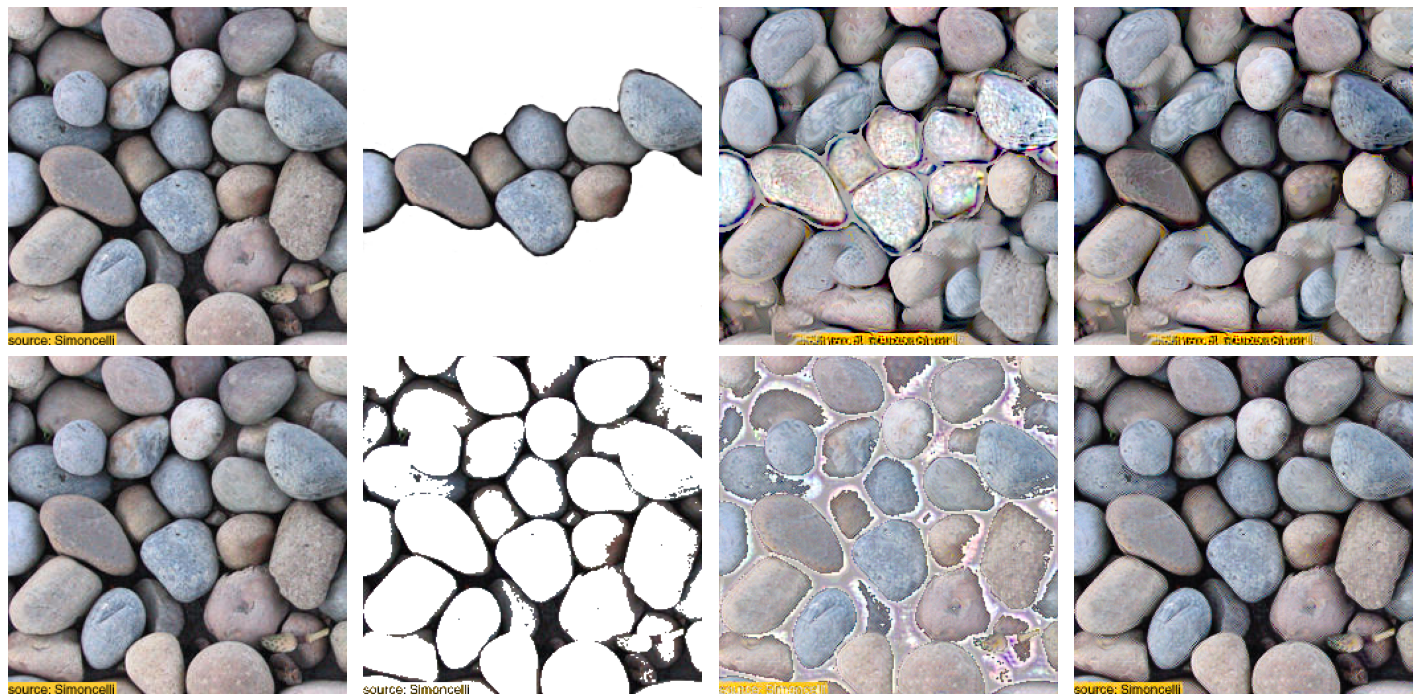
\includegraphics[width=0.8\textwidth]{images/ex01-pebbles-1000steps-crop.png}
        \caption{{\color{red} TODO: texture source? self-contained description! better figure!}}
        \label{fig:ex01-pebbles-1000steps}
    \end{center}
\end{figure}

Figure \ref{fig:ex01-pebbles-1000steps} shows the main result of this experiment. Overall, we have tested five different backgrounds and two different input texture. Complete results of those runs can be found in the appendix \ref{chapter:appendix-results}.

\subsection{Analysis}
\label{section:results-experiments-01-analysis}

\begin{figure}[ht]
    \begin{center}
        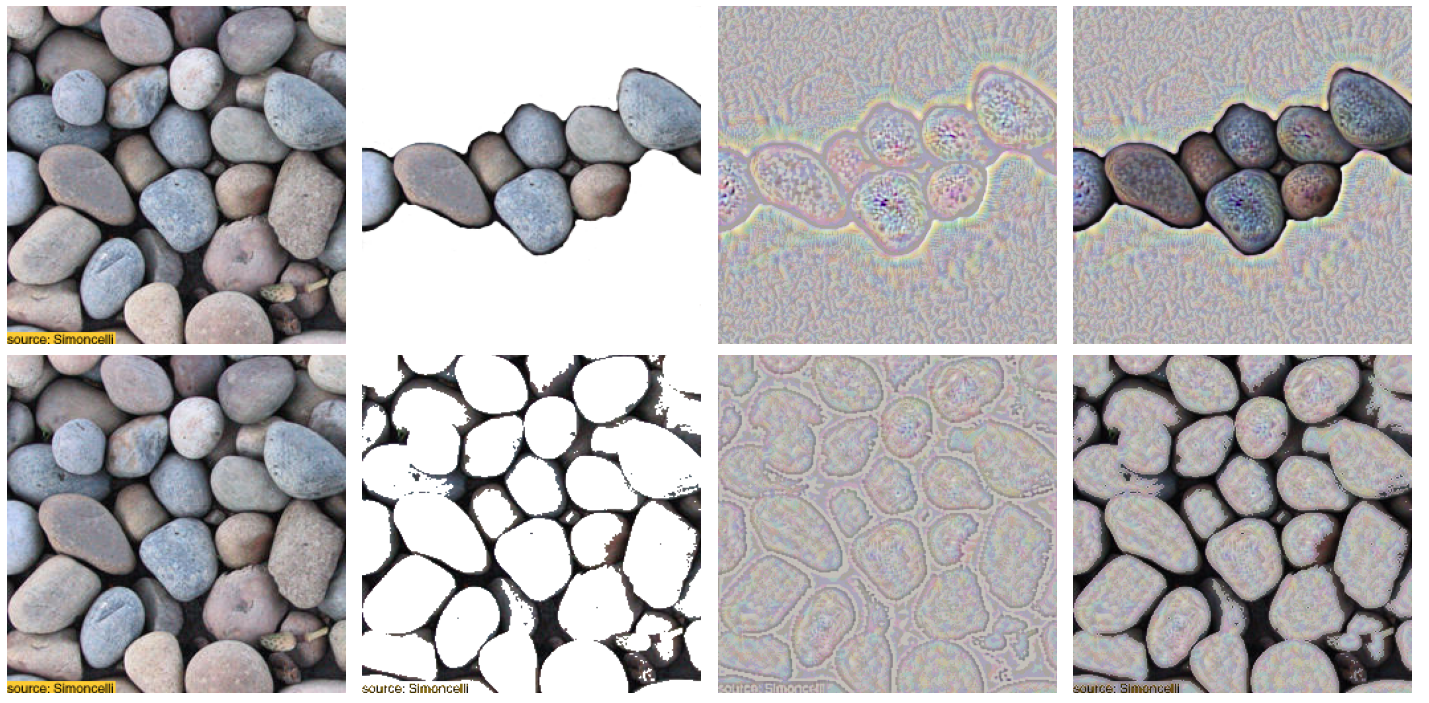
\includegraphics[width=0.8\textwidth]{images/ex01-pebbles-5steps-crop.png}
        \caption{{\color{red} TODO: texture source? self-contained description! better figure!}}
        \label{fig:ex01-pebbles-5steps}
    \end{center}
\end{figure}

It can be said that our method is indeed capable of controlling the synthesis in a way that yields those textures that match the background well. The algorithm largely respects the texture features which are already present in the background and continues the texture smoothly around them. 

Especially interesting is the second row in figure \ref{fig:ex01-pebbles-1000steps} where the outlines of all the pebbles are fixed by the background. Our method not only respects those boundaries, but also reproduces the input texture almost perfectly. This means that the second background restricts the Gatys texture model much more than the first background. ({\color{red} TODO: analyze a bit more -- micro vs. macro features, some literature, \dots})

On the other hand, in the first row of figure \ref{fig:ex01-pebbles-1000steps}, we can see that the area where the background matches the input is not fully saturated as expected. A possible explanation for this is that the algorithm starts from a white noise image with mean \(0.5\) (see figure \ref{fig:ex01-pebbles-5steps}). Combined with the fact that the loss decreases the fastest at the beginning of the optimization process ({\color{red} TODO: graph?}), this likely translated into the algorithm prefering to leave the middle area of the image darker and compensating overall brightness by making the surrounding pebbles brighter, rather than matching the exact appearance of the middle area to that of the input. From the perspective of this experiment, however, this is not a major issue.

\section{Evaluating various texture models}
\label{section:results-experiments-02}

In the first experiment (section \ref{section:results-experiments-01}), we have shown that our method is able to converge to the desired result in certain toy examples. The next step is to use more challenging situations to also evaluate how well it converges in general. 

\textbf{Goal.} We want to compare our method with traditional pixel-based projection mapping. We would also like to see the effect of various texture models on the performance of our method.

\textbf{Hypothesis.} When comparing our method with a pixel-based reference, we expect our method to perform better in challenging areas by reorganizing the input texture in a way that fits the background and therefore hides it better. When comparing original Gatys model with the improved one, we expect the improved model to be better at recovering the texture, while the original Gatys model should be more flexible in adapting to the background because its statistical texture description is less constrained.

\textbf{Setup.} We keep using the simple rendering function (see section \ref{section:methods-rendering_function-simple}) because what makes a scene challenging is the fact that the projector is forced outside its color gamut. Such conditions can be reproduced in the simplified scenario as well. As mentioned above, we use both the original Gatys texture model (see section \ref{section:methods-texture_model}) and its improved variant (\ref{section:methods-texture_model-improvements}) to compare them against each other. We obtain the pixel-based reference by removing the texture model block from our pipeline (see section \ref{chapter:methods}) and replacing it with a per-pixel L2 difference between the input texture and the optimized image. This approach yields the optimal pixel-based projection mapping algorithm without a content-based global optimization step (as described in section \ref{section:background-projection_mapping-procams-radiometric_calibration}). ({\color{red} TODO: why leave the global step out?}). The inputs to this experiment are pairs of scene (represented by a background image) and texture image that we wish to project-map.

\subsection{Results}
\label{section:results-experiments-02-results}

\begin{figure}[ht]
    \begin{center}
        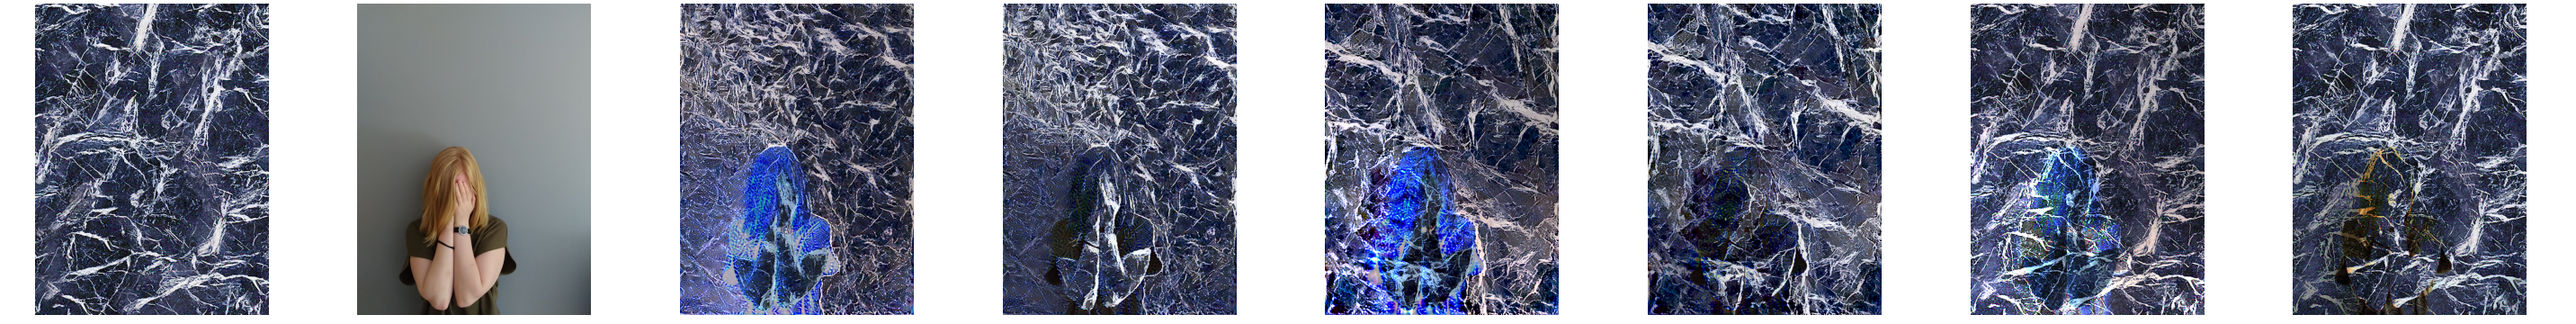
\includegraphics[width=0.95\textwidth]{images/ex02-crop.png}
        \caption{{\color{red} TODO: texture source? self-contained description! better figure! mention the brightness factor of 5 here!}}
        \label{fig:ex02}
    \end{center}
\end{figure}

Figure \ref{fig:ex02} shows the main result of this experiment. Overall, we have tested four different backgrounds and five different input textures. Complete results of those runs can be found in the appendix \ref{chapter:appendix-results}.

\subsection{Analysis}
\label{section:results-experiments-02-analysis}

\begin{figure}[ht]
    \begin{center}
        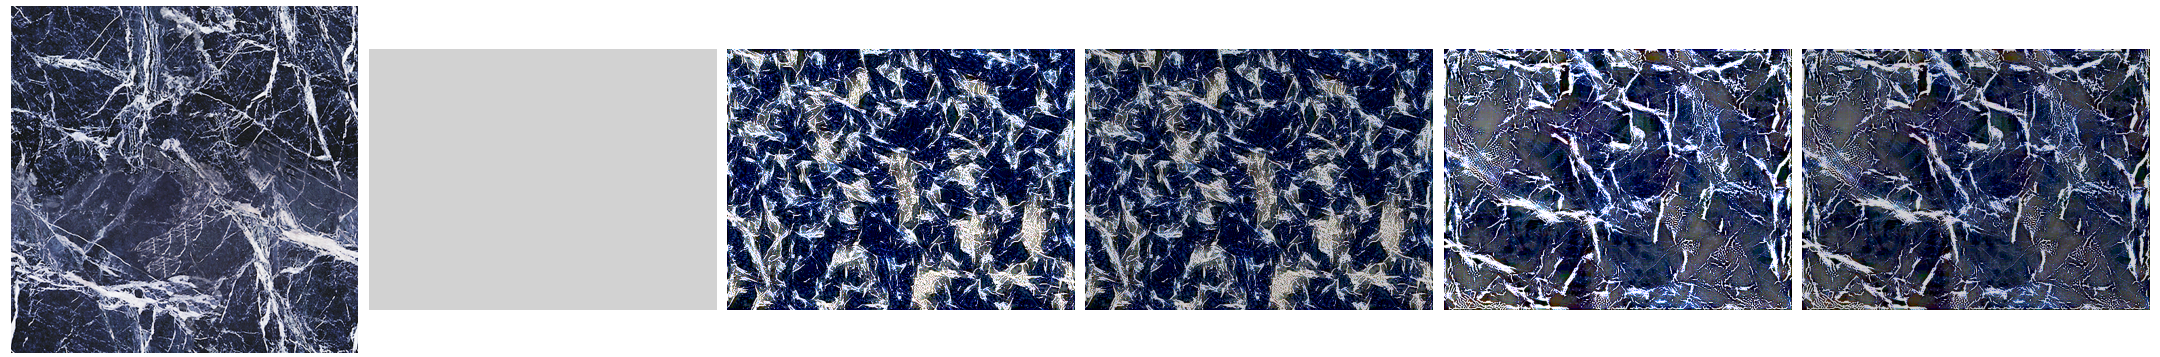
\includegraphics[width=0.95\textwidth]{images/ex02-isolating_issues-crop.png}
        \caption{{\color{red} TODO: texture source? self-contained description! better figure! compare with white background and a darker one as well! brightness factor?}}
        \label{fig:ex02-issues}
    \end{center}
\end{figure}

When comparing the three methods -- ours with Gatys texture model, ours with improved texture model and pixel-based reference -- it is useful to think in terms of microtexture and macrotexture ({\color{red} TODO: literature? Raad?}). For example, in a pebble texture like the one in figure \ref{section:results-experiments-01-results}, the pebbles themselves form a macrotexture while their surface is a microtexture.

Starting with our method with Gatys texture model, we can see that it reproduces microtexture very well. The resulting appearance mostly contains only colors from the input texture, for example hair color is completely hidden, unlike in the pixel-based reference. On the other hand, macrotexture is recovered rather poorly and its appearance seems to deteriorate in areas where the background is darker, especially in the lower left corner.

In a sense, this is an extreme case. The background in the lower left corner is clearly too dark for the projector to compensate it and at the same time it is too large for texture synthesis to place a dark part of the texture over it. On the other hand, the pixel-based reference clearly looks better in this case. Where synthesis cannot recover the color, it does not recover the macro features either, whereas the pixel-based method has the advantage of only needing to match colors and overall, darker appearance with the correct macro features looks better. We have thus conducted a separate experiment to evaluate the macro feature convergence of the two different texture models in situations where color cannot be matched. The result is shown in figure \ref{fig:ex02-issues} and suggests that the improved texture model does indeed converge a little better.

This is apparent in the main result (fig. \ref{fig:ex02}) as well. Our method with the improved texture model recovers microtexture better than the pixel-based method and its macrotexture is better than that of the Gatys texture model. Overall, we believe that our method provides a more visually pleasing and balanced result than the pixel-based reference. At the same time, the results show that even our improved texture model is not perfect and any improvements in this area should improve statistics-based projection mapping as well.

{\color{red} TODO: comparing loss values of various results sounds like an easy and useful thing to do! (e.g. compare vanilla Gram loss of a vanilla Gram results and improved result to disentange representation power and convergence)}

\section{Evaluating complex rendering function}
\label{section:results-experiments-03}

The second experiment (section \ref{section:results-experiments-02}) has shown that statistics-based projection mapping can be a viable alternative to traditional pixel-based approaches, outperforming them in certain situations. However, so far we have only tested our method in the simplified scenario of projecting on a flat diffuse surface. The last experiment represents a step towards real world deployment of our method and involves projecting onto arbitrary 3D scenes.

\textbf{Goal.} We want to see how our method copes with complex geometry and global illumination effects. These were ignored in the previous experiments where the intention was purely to stress the projector gamut. However, real scenes are full of them and our method must be evaluated in these complex scenarios as well.

\textbf{Hypothesis.} We expect the behavior from the previous experiments to translate well to a more complex setup. There is no longer a 1:1 correspondence between projector and camera pixels, but this should present no difficulty to the optimizer ({\color{red} TODO: go a little deeper here. what does it really mean mathematically to optimize using the complex rendering function?}).

\textbf{Setup.} We now finally use the complex rendering function (see section \ref{section:methods-rendering_function-complex}) in our pipeline. We also use the improved texture model and the pixel-based reference for comparison. We do not use the Gatys texture model ({\color{red} TODO: should you, though?}) because we have shown that it has issues and better models should be preferred. The inputs to this experiment are pairs of scene (represented by a pre-captured light transport matrix) and texture image that we wish to project-map. To keep the light transport matrix size manageable, we are using both projector and camera image size of \(160 \times 160\).

\subsection{Results}
\label{section:results-experiments-03-results}

\begin{figure}[ht]
    \begin{center}
        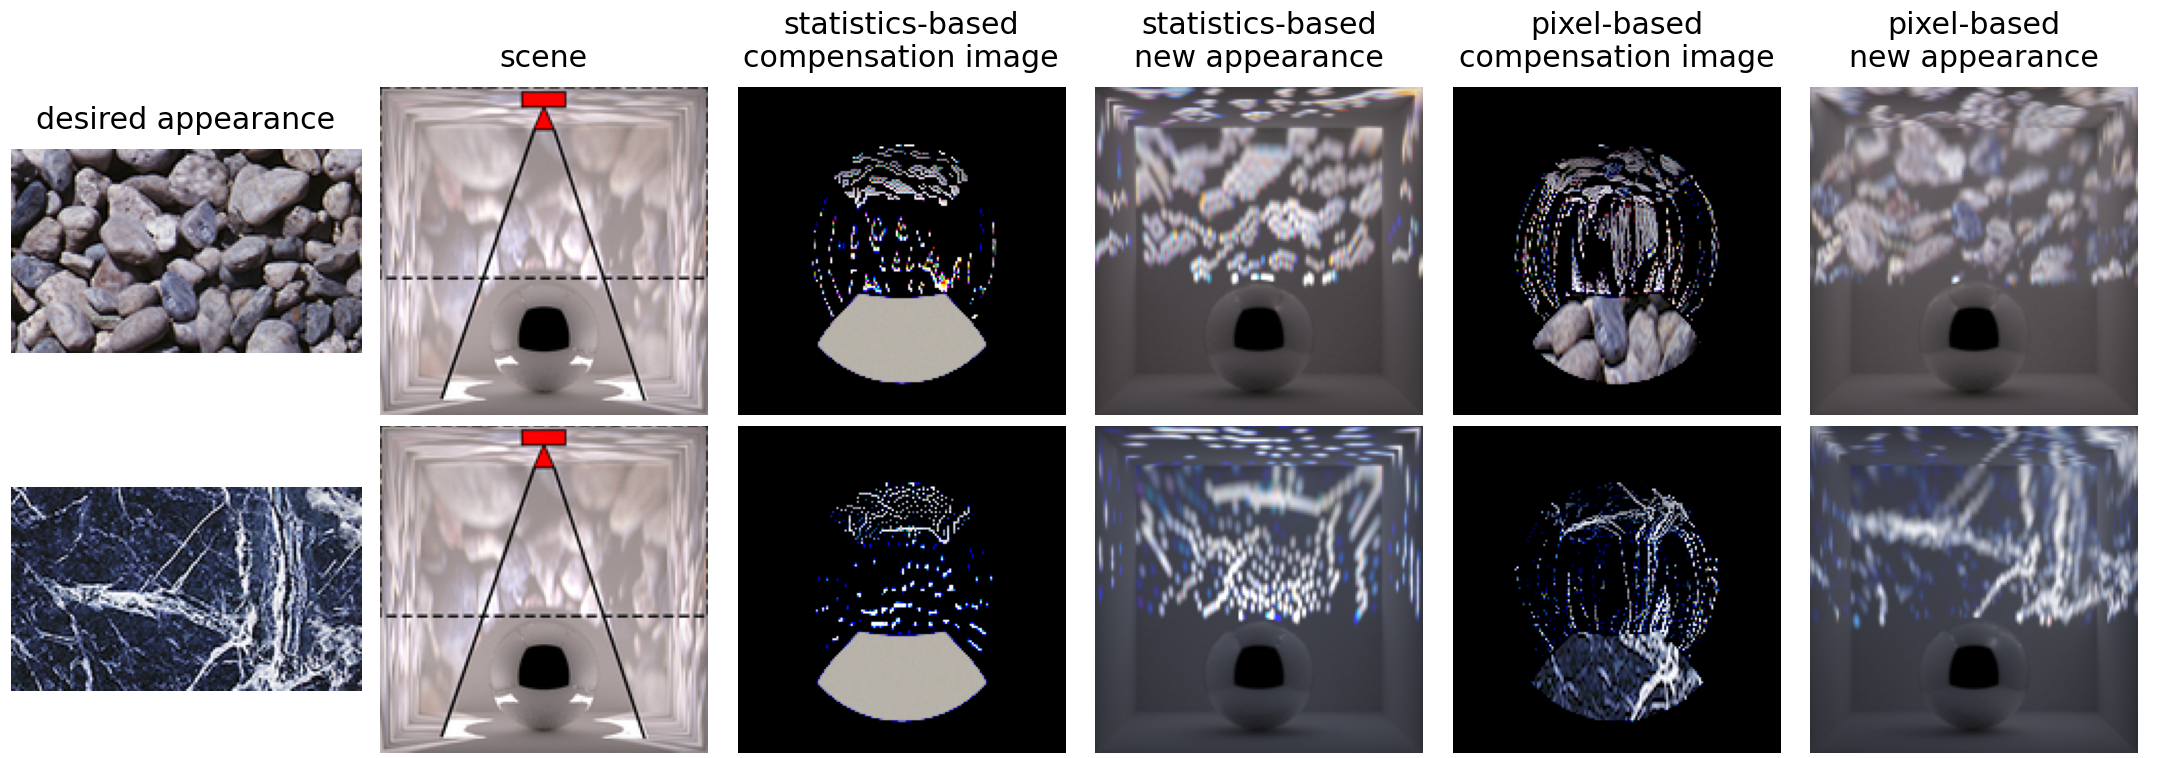
\includegraphics[width=0.95\textwidth]{images/ex03-ball-dof-crop.png}
        \caption{{\color{red} TODO: texture source? self-contained description! better figure! brightness factor!}}
        \label{fig:ex03-ball-dof}
    \end{center}
\end{figure}

\begin{figure}[ht]
    \begin{center}
        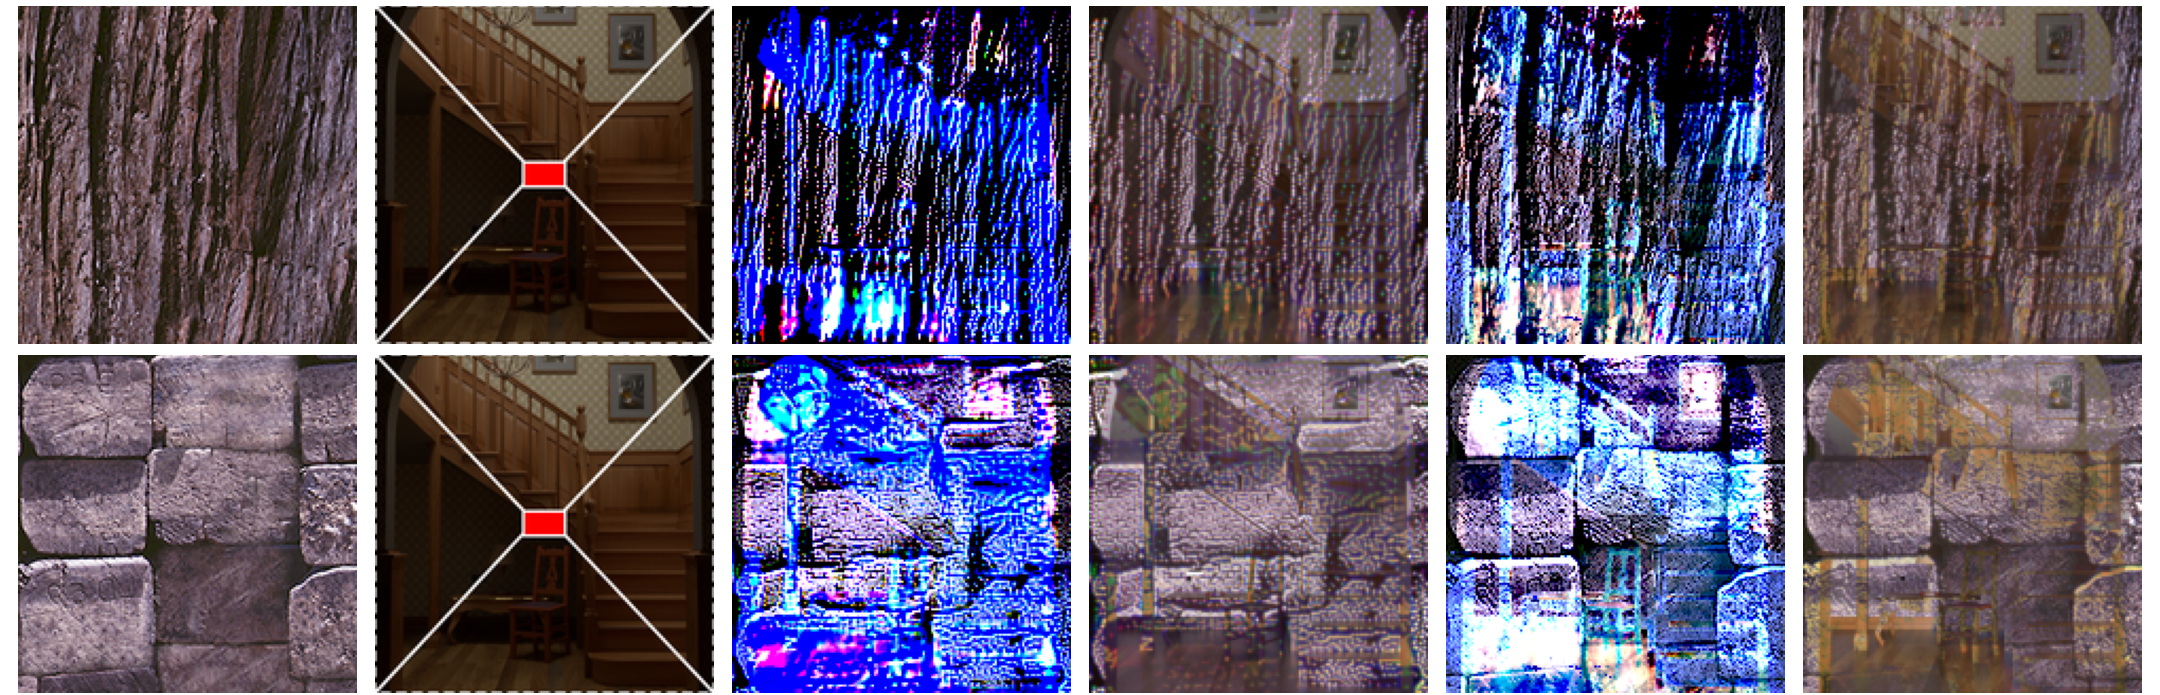
\includegraphics[width=0.95\textwidth]{images/ex03-staircase-illum-crop.png}
        \caption{{\color{red} TODO: texture source? self-contained description! better figure! brightness factor!}}
        \label{fig:ex03-staircase-illum}
    \end{center}
\end{figure}

Figures \ref{fig:ex03-ball-dof} and \ref{fig:ex03-staircase-illum} shows the main result of this experiment. Overall, we have tested two different scenes with projector DoF on and off and with and without external illumination and four different input textures. Complete results of those runs can be found in the appendix \ref{chapter:appendix-results}.

The scene used in figure \ref{fig:ex03-ball-dof} does not present any challenges regarding projector gamut, but rather it has very complicated light transport. The projector has a finite aperture which results in DoF effects and is aimed at a glass ball. The camera image is only a crop of the full view, so appearance is only optimized in the upper half of the view.

The scene in figure \ref{fig:ex03-staircase-illum} features a projector without DoF pointed at a wooden staircase. It has external illumination from a lamp above the staircase, complex textured geometry and both diffuse and glossy surfaces (floor in the lower left corner). This is a complex scene which stresses both the ability of our method to handle global illumination effects and overcome the gamut limitations of the projector.

\subsection{Analysis}
\label{section:results-experiments-03-analysis}

As we can see in both figures \ref{fig:ex03-ball-dof} and \ref{fig:ex03-staircase-illum}, our method handles the complex relationship between projector pixels and camera pixel well and its performance on 3D scenes is comparable to that on simple flat surfaces. Compared to the pixel-based reference, it performs worse in recovering the macro features, but it is better at recovering microtexture. For example, in the staircase scene \ref{fig:ex03-staircase-illum} in the lower left, the input texture is very bright, but the scene contains a glossy floor which is difficult to project onto. Whereas the pixel-based reference struggles to achieve the desired appearance and oversaturates corresponding projector pixels, our method instead moves the darker part of the texture into this area which provides a more satisfying result.

{\color{red} TODO: projecting normal compensation via DoF matrix and vice-versa might a very cool thing to do! Also the same with illuminated/non-illuminated staircase. In general, this section would probably benefit from some discussion on at least the compensation of the DoF effect}

{\color{red} TODO: about the resolution issue: might be better to leave it for the conclusion}